\chapter{观测量、关联函数与误差条}
\label{ch:observables}

\begin{learningobjectives}
完成本章后，读者应能：
\begin{enumerate}
  \item 把 Wigner 轨迹上的对称排序量转换为正规排序观测量；
  \item 构造密度、一体相干、二阶关联、动量分布和结构因子；
  \item 为非线性与比值估计器计算不过度乐观的统计不确定度；
  \item 区分 Monte Carlo 误差、数值系统误差与方法误差。
\end{enumerate}
\end{learningobjectives}

\section{轨迹变量不是观测量本身}

Wigner 平均天然对应对称排序。实验和多体理论中常见的密度、粒子数和光子计数则是正规排序。第4章已经给出单模例子；对有限模式场，所有修正都由投影核 $\delta_{\mathcal C}(x,x')$ 决定。
相空间排序对应的系统综述见\cite{Hillery1984}；多分量投影场中的 functional
Wigner 估计器可与\cite{Opanchuk2013}核对。

一个稳健的分析流程应把三层对象分开：
\begin{enumerate}
  \item \textbf{原始轨迹量}，例如 $|\psi^{(s)}(x,t)|^2$；
  \item \textbf{逐轨迹或系综估计器}，包含排序修正；
  \item \textbf{最终统计量}，包含归一化、比值、拟合和置信区间。
\end{enumerate}
若把修正散落在绘图脚本中，同一数据很容易被两次扣除半量子或完全不扣除。

\section{密度与一体相干}

正规排序一体密度矩阵为
\begin{equation}
  G^{(1)}(x,x';t)
  =\qavg{\hpsid(x,t)\hpsi(x',t)}.
\end{equation}
其 Wigner 估计器是
\begin{equation}
  G^{(1)}(x,x';t)
  \approx
  \ensavg{\psi^*(x,t)\psi(x',t)}
  -\frac12\delta_{\mathcal C}(x,x').
  \label{eq:g1-wigner-estimator}
\end{equation}
令 $x'=x$ 得密度
\begin{equation}
  n(x,t)=\ensavg{|\psi(x,t)|^2}
  -\frac12\delta_{\mathcal C}(x,x).
  \label{eq:density-wigner-estimator}
\end{equation}
对正交格点，$\delta_{\mathcal C}(x_j,x_k)=\delta_{jk}/\Delta x$。不同格点的一体相干没有局域半量子扣除；同一点则必须扣除。

归一化一阶相干度通常定义为
\begin{equation}
  g^{(1)}(x,x')=
  \frac{G^{(1)}(x,x')}{\sqrt{n(x)n(x')}}.
  \label{eq:normalized-g1}
\end{equation}
应先分别估计分子和密度，再取比值；逐轨迹计算
$\psi^*(x)\psi(x')/[|\psi(x)||\psi(x')|]$ 回答的是相位因子问题，并不等于式\eqref{eq:normalized-g1}。

\section{二阶正规排序关联}

局域二阶关联的未归一化分子为
\begin{equation}
  G^{(2)}(x,x)
  =\qavg{\hpsid(x)^2\hpsi(x)^2}.
\end{equation}
对应的有限模式 Wigner 估计器是
\begin{equation}
  G^{(2)}(x,x)
  \approx\ensavg{
  |\psi|^4-2\delta_{\mathcal C}|\psi|^2
  +\frac12\delta_{\mathcal C}^2},
  \label{eq:local-g2-wigner-estimator}
\end{equation}
其中投影核均取 $(x,x)$。归一化二阶相干度为
\begin{equation}
  g^{(2)}(x,x)=\frac{G^{(2)}(x,x)}{n(x)^2}.
  \label{eq:normalized-g2}
\end{equation}
式\eqref{eq:local-g2-wigner-estimator}不是
$(|\psi|^2-\delta_{\mathcal C}/2)^2$；后者常数项为
$\delta_{\mathcal C}^2/4$，少了四次算符 Weyl 符号要求的另一项。

一般两点的正规排序分子
$G^{(2)}(x,x')=\qavg{\hpsid(x)\hpsid(x')\hpsi(x')\hpsi(x)}$
还包含非局域投影核。把所有场与投影核取在同一时刻，其 Wigner 估计器为
\begin{equation}
  G^{(2)}(x,x')\approx\ensavg{\begin{aligned}
  &|\psi(x)|^2|\psi(x')|^2
  -\frac12\delta_{\mathcal C}(x,x)|\psi(x')|^2
  -\frac12\delta_{\mathcal C}(x',x')|\psi(x)|^2 \\
  &-\frac12\delta_{\mathcal C}(x,x')\psi^*(x')\psi(x)
  -\frac12\delta_{\mathcal C}(x',x)\psi^*(x)\psi(x') \\
  &+\frac14\delta_{\mathcal C}(x,x)\delta_{\mathcal C}(x',x')
  +\frac14|\delta_{\mathcal C}(x,x')|^2
  \end{aligned}}.
  \label{eq:nonlocal-g2-general}
\end{equation}
令 $x'=x$ 即恢复式\eqref{eq:local-g2-wigner-estimator}。这一完整形式在
非正交投影基中尤其重要：即便两个坐标点不同，投影核也未必为零。

对两个不同的正交格点 $j\neq k$，正规排序关联可写成
\begin{equation}
  G^{(2)}_{jk}
  =\frac{1}{\Delta x^2}
  \ensavg{
  \left(|\alpha_j|^2-\frac12\right)
  \left(|\alpha_k|^2-\frac12\right)}.
  \label{eq:nonlocal-g2-grid}
\end{equation}
当 $j=k$ 时必须改用式\eqref{eq:local-g2-wigner-estimator}，因为同一模式的算符收缩多出接触项。

\section{动量分布与 Fourier 约定}

在 $M$ 点周期格点上定义归一化离散变换
\begin{equation}
  \alpha_\ell^{(k)}=\frac{1}{\sqrt M}
  \sum_{j=0}^{M-1}\ee^{-2\pi\ii j\ell/M}\alpha_j,
  \qquad
  \alpha_j=\sqrt{\Delta x}\,\psi_j.
  \label{eq:unitary-discrete-fourier}
\end{equation}
该变换保持 $\sum_j|\alpha_j|^2=\sum_\ell|\alpha_\ell^{(k)}|^2$。每个保留动量模式的占据为
\begin{equation}
  n_\ell^{(k)}=\ensavg{|\alpha_\ell^{(k)}|^2}-\frac12.
  \label{eq:momentum-occupation-estimator}
\end{equation}
许多数值 FFT 默认没有式\eqref{eq:unitary-discrete-fourier}的 $1/\sqrt M$ 对称归一化。代码必须在单模平面波上验证：实空间总粒子数、动量空间占据之和和 Parseval 恒等式三者一致。

连续动量密度 $n(k)$ 还涉及 Fourier 变换中的 $2\pi$ 约定及 $k$ 格距，不能仅把数组 $|\mathrm{FFT}(\psi)|^2$ 标成“占据”。正文、代码和图轴应明确画的是每个离散模式的粒子数还是单位波数的粒子密度。

\section{密度涨落与结构因子}

定义 $\delta\hat n(x)=\hat n(x)-n(x)$。静态结构因子可写成
\begin{equation}
  S(k)=\frac{1}{N}\int\dd x\dd x'\,
  \ee^{-\ii k(x-x')}
  \qavg{\delta\hat n(x)\delta\hat n(x')}.
  \label{eq:static-structure-factor}
\end{equation}
对第10章的投影场，密度算符乘积满足
\begin{equation}
  \qavg{\hat n_{\mathcal C}(x)\hat n_{\mathcal C}(x')}
  =G^{(2)}_{\mathcal C}(x,x')
  +\delta_{\mathcal C}(x,x')G^{(1)}_{\mathcal C}(x,x').
  \label{eq:density-shot-noise}
\end{equation}
右端第二项是粒子散粒噪声。在完整连续基极限，它退化为
$\delta(x-x')n(x)$。对均匀连续体系的非零波数，常用形式为
\begin{equation}
  S(k)=1+\frac{1}{N}\int\dd x\dd x'\,
  \ee^{-\ii k(x-x')}
  \left[G^{(2)}(x,x')-n(x)n(x')\right].
  \label{eq:structure-factor-normal-ordered}
\end{equation}
若用正规排序 $G^{(2)}$ 构造式\eqref{eq:structure-factor-normal-ordered}，就必须保留前面的 $1$；若直接从完整密度--密度关联出发，则不能再额外添加它。对有限投影基，应按式\eqref{eq:density-shot-noise}显式计算投影后的散粒噪声项，不能不加检查地把它替换成 $1$。

有限且不均匀体系的 $k=0$ 分量还包含总数涨落和非零平均密度 Fourier 分量，应使用式\eqref{eq:static-structure-factor}逐项计算，不宜套用均匀简式。

\section{序参量、条纹和有限尺寸}

密度波的复振幅可以定义为
\begin{equation}
  \rho_Q=\frac{1}{N}\int\dd x\,
  \ee^{-\ii Qx}n(x).
  \label{eq:density-wave-amplitude}
\end{equation}
若哈密顿量保持平移对称，而有限轨迹在随机位置形成条纹，系综平均 $\ensavg{\rho_Q}$ 可以因随机相位为零。此时
$\ensavg{|\rho_Q|^2}$ 或 $S(Q)$ 能检测有限尺寸密度关联，但其非零本身不证明热力学极限自发对称破缺。还需要随系统尺寸、粒子数、显式钉扎场和观测时间做标度。第17章将把这一点与超流响应结合。

相似地，先对每条轨迹寻找最大峰再平均会产生选择偏差，即使纯噪声也给出正“条纹对比度”。若峰位不是理论预先给定，应在独立数据上选窗，或把寻峰步骤完整纳入空模型与 bootstrap。

\section{统计误差条}

对 $N_s$ 条独立轨迹的标量估计器 $X_s$，样本均值和标准误为
\begin{equation}
  \bar X=\frac{1}{N_s}\sum_sX_s,
  \qquad
  {\rm SE}(\bar X)=
  \sqrt{\frac{1}{N_s(N_s-1)}\sum_s(X_s-\bar X)^2}.
  \label{eq:monte-carlo-standard-error}
\end{equation}
误差条反映有限轨迹，不包括时间步长、截止或 TWA 截断误差。

对 $R=A/B$、$g^{(2)}=G^{(2)}/n^2$ 等非线性统计量，不应先算每条轨迹的比值再平均。应从全体样本估计 $A,B$ 后取比值，并用按轨迹重抽样的 bootstrap 或 jackknife 传播其相关性。若 $B$ 接近零，比值分布可能强烈偏斜，此时对称的“均值正负一个标准差”会误导，应报告分位数区间或停止解释该区域。

空间格点和同一轨迹的多个时刻不是独立 Monte Carlo 样本。bootstrap 的基本重抽样单元应是完整轨迹；若初态来自 Markov 链，还须按自相关时间分块。

\section{多时关联的额外困难}

等时对称排序量可以直接由同一时刻轨迹计算。不同时间的普通量子乘积如
$\qavg{\hpsid(t)\hpsi(t')}$ 涉及算符顺序与响应，通常不等于简单的
$\ensavg{\psi^*(t)\psi(t')} $。受控计算可能需要 Bopp 算符、对初始条件的切线响应，或 Schwinger--Keldysh 路径上的插入。若只采用经典轨迹乘积，应明确它近似的是哪种半经典相关函数，不应默认为任意量子时间排序。

最简单的谐振子已经能看出差别。若
$\hat a(t)=\ee^{-\ii\omega t}\hat a(0)$，初态平均占据为 $\bar n$，则
\begin{align}
  \ensavg{\alpha^*(t)\alpha(t')}
  &=\left(\bar n+\frac12\right)\ee^{-\ii\omega(t'-t)},\\
  \qavg{\had(t)\ha(t')}
  &=\ensavg{\alpha^*(t)\alpha(t')}
  -\frac12\ee^{-\ii\omega(t'-t)}.
  \label{eq:two-time-harmonic-ordering}
\end{align}
这里的第二项是传播后的对易子，而不是只在 $t=t'$ 才出现的常数。对
非线性轨迹，该修正一般依赖切线响应
$\partial\alpha(t')/\partial\alpha(t)$，不能由一个通用的“减半量子”
规则替代。因此本书配套观测量程序只验证等时单模估计器；它没有验证
空间关联或任意多时量子关联。

\section{实际排序估计器基准}

配套程序分别抽样平均占据为 $4$ 的相干态和平均占据为 $2$ 的热态，用同一批轨迹计算密度、四阶正规排序矩与 $g^{(2)}$，结果见\cref{fig:ordering-estimator-benchmark}。
\begin{figure}[htbp]
  \centering
  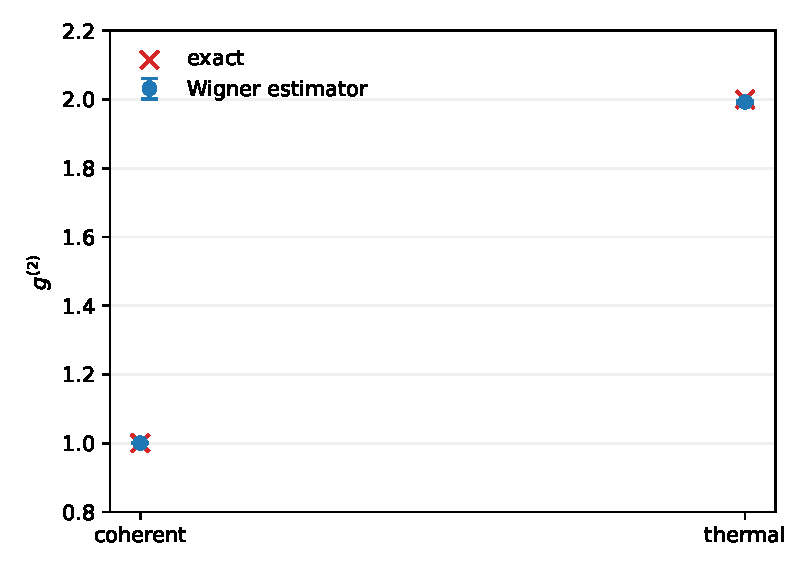
\includegraphics[width=0.72\textwidth]{figures/ch13/ordering_estimators.pdf}
  \caption[相干态与热态的正规排序估计器基准]{正规排序估计器的单模基准。相干态（$\bar n=4$）与热态（$\bar n=2$）各使用 $400000$ 个样本；$g^{(2)}$ 误差棒为 $200$ 组 jackknife 得到的 $\pm1$ 标准误。估计值分别为 $1.0002\pm0.0006$ 与 $1.9927\pm0.0049$，与解析值 $1$、$2$ 相容。该图不构成非局域关联、结构因子或多时响应实现的验证。}
  \label{fig:ordering-estimator-benchmark}
\end{figure}
相干态解析值为 $g^{(2)}=1$，热态为 $g^{(2)}=2$。程序使用分组 jackknife 给比值误差条，实际指标保存于
\path{data/ch13/ordering_estimator_metrics.json}。
这是排序公式的单模单元测试，不应被解释为式
\eqref{eq:nonlocal-g2-general}、结构因子或多时响应实现已经通过端到端验证。

\begin{chaptercheck}
为每张结果图附一张内部“误差预算表”：列出排序公式、轨迹数与统计误差、步长变化、截止变化、计算域变化和独立方法比较。最终正文可以压缩该表，但原始记录应保留，以免把很小的 Monte Carlo 误差条误当作总可信区间。
\end{chaptercheck}

\section*{本章小结}

Wigner 轨迹必须经过与算符排序相匹配的估计器才能变成物理观测量。密度扣除半个投影模式基线，局域四阶关联包含不同的二次与常数修正，结构因子还要正确处理散粒噪声。比值、寻峰和多时关联具有额外统计或算符顺序风险。轨迹误差条只度量 Monte Carlo 不确定度，不能覆盖数值、截止和方法误差。

\begin{exercises}
  \item 从单模四次算符的 Weyl 符号推导式\eqref{eq:local-g2-wigner-estimator}。
  \item 证明式\eqref{eq:unitary-discrete-fourier}保持原始对称范数
  $\mathcal N_{\mathrm{sym}}$，并说明固定模式数时为何也保持 $N_W$。
  \item 对相干态与热态分别计算 $g^{(2)}(0)$ 的解析值。
  \item 构造一个分母接近零的比值估计例子，比较 delta 方法与 bootstrap 区间。
  \item 说明为什么在每条噪声轨迹中搜索最大 Fourier 峰会产生正偏差，并设计一个空模型校准。
\end{exercises}
